%!TEX root = ../Masterthesis.tex
\chapter{Tracking in real space}
The previous sections provided information on the structure of the human hand and how to represent it in the digital space. To apply the algorithms presented in Section \ref{kinematics} to our digital hand model, we need input data from our real world representative.
\section{General tracking technologies}
\label{General tracking technologies}
The methods for gaining positional data can be roughly categorized into two major groups, glove based methods and vision based methods. Glove based methods have already been in developement since the 1980's \cite{Bolt.1980} and have since then resulted in several solution attempts. Sturman and Zeltzer gave a survey on the exsisting tracking mehtods in their paper \cite{Sturman.1994}. \\They distinguish between two areas of tracking, first the 3D positional tracking of the hand (and also other bodyparts) without regard to the hands shape and secondly the tracking of the hand shape with glove technologies.\\These tracking technologies presented are still applied today in modern tracking solutions \cite{Welch.2002,Rolland.2001}. They account for solutions based in optical tracking based on marker detection, magnetic detection via measurements of an artificial magnetic field\cite{Raab.1979} and accoustic measurements via triangulaton of ultrasonic pings.

\subsection{Optical tracking}

The components for an optical tracking systems are several cameras for object detection and some kind of tracking characteristic of the object to be tracked. These characteristics can be either artificially applied ones like active flashing infrared LED on key tracking positions of the body or infrared reflective markers.\\ A series of cameras positioned around the tracking subject will then track these markers inside their visual fields. The second method uses a single camera to capture the silhouette image of the subject, which is analyzed to determine positions of the various parts of the body and user gestures.
\\The image data is supplied to special software which correlates the marker positions in the multiple viewpoints and uses the different lens perspectives to calculate a 3D coordinate for each marker. These image interpretation and correlation tasks require computationally costly operations. The marker tracking is also prone to errors through variation in lighting of the scene, material reflection properties and also marker occlusion as the trackers are moved. Also most of the systems rely on several tracking cameras for a complete coverage of the tracking space. This leads to a higher system complexity in terms of setup and calibration.
\begin{figure}[H]
\label{optic reflector tracking}
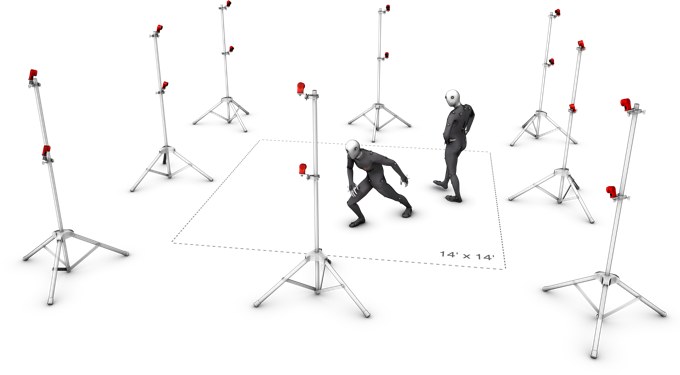
\includegraphics[scale=0.6]{images/flex13MocapVolume.png} 
\caption{Example for an optical tracking system with passive infrared reflector markers \cite{optitrack.2017}}
\end{figure}
\subsection{Magnetic tracking}
The usage of a magnetic field for position tracking is a relatively uncomlicated technique. The earth already provides us with a magnetic field to orient on. Simular to the optical trackers, magnet field sensors can be placed at key tracking positions. These sensors measure field strength in 3 orthogonally orented axes to produce a 3D vector of the unit’s orientation with respect to the excitation. As the earths magnetic field prone to changes based on geographical location, data corrections have to be applied to the measurements.\\Another solution is to generate an local magnetic field via a multicoil source unit. The source unit coils are energized in sequence and the corresponding magnetic field vector is measured in the sensor unit. With three such excitations, you can estimate the position and orientation of the sensor unit with respect to the source unit.\\the downside of this technology is that ferromagnetic and conductive material in the surrounding environement will have an effect on the generated magnetic field. These distortion effects will form small unwanted secondary source units through the induction of small Foucault currents by the main sources magnetic field.
Magnetic fields have the property of having an inverse cubic falloff  as a function of distance from the source, which limits the rango of operation for the system.
Position resolution in the radial direction from source to sensor depends on the gradient of the magnetic field strength, and thus the positional jitter grows as the fourth power of the separation distance.\\
In comparison to other tracking technologies, the magnetic field tracking solution has the conveniece of not suffering from line of sight problems from tracker occlusion. The magnetic fields are capable of passing through the human body. Also the sensor size for measuring magnetic fields is rather small, giving the trackers a small volume. Furthermore, only one source unit is needed for the tracking of multiple sensor units.
\subsection{Accoustic tracking}
The principles of accoustic tracking are very simular to those of the optic tracking technologies. Instead of using lightwaves, the systems utilize acoustic pulses of ultrasonic wavelenghts to time the time of flight between emitter and sensor for range measurement. To get a good measuring result from the systems, the used accoustic transducerst have to be as omnidirectional as possible,so that the signal can be detected no matter how the emitter is positioned or oriented in the tracking volume. For the speakers to acchieve a wide beam width, their size has to be small.\\ To be able to build the microphones into the tracker, they can only have active surfaces a few millimeters in diameter. This leads to a reduction in range as the efficiency of accoustic transducers is proportial to the active surface area. Also accoustic systems can have problems with ambient noises occluding the signal. This becomes even mor critical when using such a system outdoors.\\Soundwaves travel at a much slower speed than lightwaves which brings benefits and downsides with it. Soundwaves can be reflected from objects, producing so echos which arrive at the recieving sensor at a later point in time. Here the slower speed can be beneficial as we can await the first sound occurence to arrive at the sensor and filter out all later reflections from the data. The reflections of the previous pluse also have to be subsided before a new measurement can be made, lowering the uodate rates of the system. The air the soundwaves travel through is also a limiting factor as humidity, airpressure and air currents can influence the travelling soundwaves.In comparison to the optical systems, the accoustic systems are not as prone to occlusion errors since soundwaves have a better ability to bend around obstacles  than lightwaves.
\\Most of these downside can be adressed with a combination of these systems with another form of tracking like in \cite{Foxlin.1998}.
\section{Hand tracking Systems}
\label{hand-tracking_systems}
In comparison to the tracking of the whole human body, the tracking of the human hands with their maximum of 27 DoF's each in a small space is rather difficult to handle.\\
The systems that try to achieve this have to encounter several difficulties. Self occlusion also plays a great role in the system design, especiall when working with only one tracking optical system for reduced complexity. Also these systems need to maintain a certain amount of processing speed for achieving a fluent reproduction of the captured motion. This demands the capability of processing large amounts of data in very short intervals. Most prototype testing for the described systems will be done in an controlled environement where the background is known. For a more widespread use, these systems need to be capable of registering the hand on an unrestricted background, which may have a wide range of patterns, color and lighting differences. Also human hand motion itsself is quite fast, resulting in a higher framerate demand for the tracking cameras.\\
The following section will describe different approaches to solve the aforementioned difficulties.

\subsection{Sensor based}
\label{Sensor based}
Tracking systems thath make use of sensors mounted to the hand via straps or a glove have alread been in use since the 1970's. First prototype glove systems included the Sayre Glove\cite{ThomasA.DeFanti.1977} and the Digital Entry Data Glove\cite{Grimes.1983}.\\
The Sayre glove is based off an idea of Richard Sayre. The system utilizes a light sourec and a photocekk which are connected via a flexible tube. These components are mounted along each finger of the hand. The light that passes through the tube is infulenced by the bending angle of the tube which corresponds to the finger bending.
a large bending angle of the finger induces a larger bending angle of the tube, reducing the intensity of the light that reaches the photodiode. The resulting voltage in the photocell can then be mapped to a specific bending angle of the finger.\\
The Digital Entry Data Glove was patented by Gary Grimes in 1983. Instead of using only one type of sensors for measurement, this glove based systems used several sensor types for different measurements.
Touch or proximity sensors were used for determining whether the user’s thumb was touching another part of the hand or fingers. To measure the flexion of the joints in the thumb, index, and little finger four “knuckle-bend sensors” were used.
\begin{wrapfigure}[11]{r}{5cm}
\label{acceleglove}
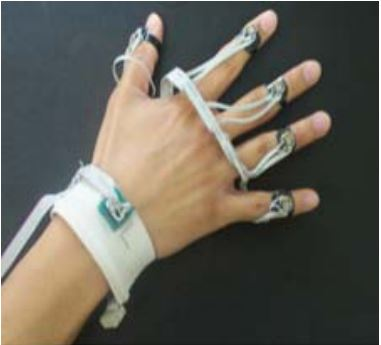
\includegraphics[scale=0.5]{images/acceleglove.JPG} 
\caption{Acceleglove system with the described sensor positions \cite{HernandezRebollar.2002}}
\end{wrapfigure}
To get measurements  for the tilting of the hand in respect to the horizontal plane two tilt sensors were mounted. Finally two inertial sensors for measuring the twisting of the forearm and the flexing of the wrist were utilzed.This glove was intended for creating “alphanumeric characters” from hand positions. Recognition of hand signs was performed via a hard-wired circuitry, which mapped 80 unique combinations of sensor readings to a subset of the 96 printable ASCII characters.
\\These early systems only provided a limited amount of sensors and were rather unpractical in usse. As they were developed to serve very specific applications,  they were used only briefly, and never commercialized.
\\Newer developements in this sector include \cite{Kuroda.2004,HernandezRebollar.2002,Majeau.2012}. The \textit{AcceleGlove} presented by \cite{HernandezRebollar.2002} consistsis  of six dual-axis accelerometers, mounted on the fingers and the back of the palm, reporting position with respect to the gravitational vector. Sensors are placed on the back of the middle phalanges, on the back of the distal phalange of the thumb, and on the back of the palm.\\
Kuroda et al \cite{Kuroda.2004} introduced the \textit{StrinGlov}, which obtains full degrees of freedom of human hand using 24 Inductcoders and 9 contact sensors, and encodes hand postures into posture codes on its own DSP. The bending angles of the fingers are measured with the inductcoders. These sensors realte the finger movement to a change in magnetic flux induced by the movement of the sensor parts thath are attached to the finger. The sensor functionality is simular to the functionality of the light sensors from  \cite{ThomasA.DeFanti.1977}. The 9 contact sensors, also based on magnetic fields,  are put on the fingertips and on the inside of the hand to be able to measure contact between two fingetips or the fingertips and the hand. The system furthermore benefits from simple structure, which leads to low production cost. 
Majeau et al \cite{Majeau.2012} propsed a systems that uses optical flexion sensors to determine the bending angles of the fingers. The opticcal flexion sensors consist of a LED, a Photodetector and an optical fibre. The LED emits light which travels through the optical fibres and the intensity that results as the output from the fibre end is measured by the Photosensor. This measuring principle also corresponds to the principle of \cite{ThomasA.DeFanti.1977}. Furthermore the system is also capable of measuring the abduction of two finger. Here the LED is mounted to one finger and the detector on the other. The optical fiber is run from the LED down the finger to the knucklebase and then up to the detector. When abducting the two fingers, the angle at the knucklebase changes, resulting in an intensity change at the detector through the loss of intensity at the curvature of the optic fibre.
The cange in intensity of both measurting techniques can be mapped to corresponding hnd movements.
\\Further readings on sensor based hand tracking systems can be found in \cite{Dipietro.2008,Sturman.1994}
\todo{Find 1-2 newer systems for comparison}

\subsection{Appearance Based - Optical marker}
\label{Appearance Based Optical marker}
Optical approaches use properties of the human hand to hand to estimate the current position. The evaluation of the hand pose is usually split up into two steps. The first one is the registration of the "real" hand.\\
\begin{wrapfigure}[7]{r}{0.52\textwidth}
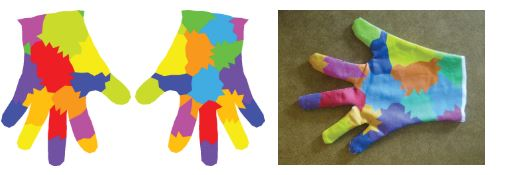
\includegraphics[scale=0.61]{images/wang_color_glove.JPG}
\caption{Color glove setup used by Wang and Popovic \cite{Wang.2009} }
\label{wang color glove}
\end{wrapfigure}
This is mostly done by at least one camera which is aimed at the hand, supplying a "continous" data stream to the evaluation Software. In the secinbd step, the evaluation software then tries to find key spots in the provided images. This data is then used for the search of the mathcing digital pose. The definition of these key spots can be achieved by several techniques.\\
An example is the usage of some kind of marking for finger segments as displayed in \cite{Duca.2007,Fredriksson.2008,Wang.2009}.
In the method described by Wang and Popovic \cite{Wang.2009},a specially colored glove is used. The glove is segemnted into ten segments, colored randomly from a pool of ten distinct colors (see Figure \ref{wang color glove}).

\begin{wrapfigure}[13]{r}{0.42\textwidth}
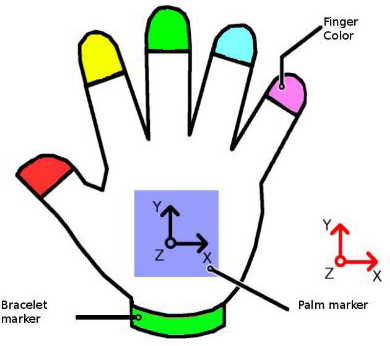
\includegraphics[scale=0.61]{images/fredrikkson_color_glove.JPG}
\caption{Color glove setup used by Fredriksson and Ryen \cite{Fredriksson.2008} }
\label{Fredriksson color glove}
\end{wrapfigure}

The pattern is createdby selecting twenty seed triangles on a 3-D hand model that are maximally distant from each other. The remaining triangles are assigned into patches based on their distance to each of these seeds. Each patch is assigned one of the ten colors at random. The jagged boundaries between the patches are artifacts from the low triangle count of the used hand model.
Algortihms that use other characteristics for tracking like texture or shading \cite{LaGorce.2008} rely on an acurate pose from a previous frame to constrain the posure search in the current frame. When using bare hand pose estimation two different handposes can map to similar images. This can lead to an inacurate pose estimation and the breakdown of the algorithm if the wrong estimation is made.
The benefit of the color glove is that the unique patch pattern, hand poses always map to ditinguishable images, simplifying the search process. Therefore it can effectively recover itsself at each frame without the need of a previous frame.
With the colored glove as a tracking feature, the images from the camera are prepared for a database sampling step. The database that was used consisted of 18,000 finger configurations. 
A distance metric between two configurations was defined as the root mean square (RMS) error between the vertex positions of the corresponding skinned hand models. With this distance metric, a low dispersion low-dispersion sampling was used to draw a uniform set of samples from the overcomplete collection of finger configurations.
The selected configurations are rendered at various 3-D orientations using a (synthetic) hand model at a fixed position from the (virtual) camera.
The camera image was compared then compared to the databse iamges. The comaprison is done via a nearest neighbor lookup using a Hausdorff-like distance \cite{Huttenlocher.1993} and penalizing the distance to the closest pixel of the same color in the other image.The resulkting pose from the database can then be applied to the digital hand model.
The method presented by Fredriksson and Ryen \cite{Fredriksson.2008} also uses a color coded glove. In constrast to the fully colored glove described before, the used glove only has colored fingerstips, color markers for the palm and a colored band for the wrist.

The palm markers and the wrist band are used to retrieve the 3D position of the hand. The wrist marker is furthermore used to define the bondingbox of the the tracking area in a calibration process. Defining a bounding greatly simplifies further image analysis operations by taking away a large amount of uneeded image data.
After determining position and orientation of the hand in 3d by utilizing wrist band an palm marker position, the system tracks the grip angle and the lateral tilt angle for each finger. The grip angle is defined as as the curling of the finger towards the palm.The second angle is defined as the lateral tilt angle which measures the spread of the fingers.
The grip angle is calulated by comparing the density of finger pixels around an estimated knuckle line. from the density, an estimations for
the finger’s Y position around an origin position at the knuckle’s base is made. This value is then transformed into an angle value using an inverse tangent operation.

One downside of this tracking method is that it does not yet incoorporate the movement of the thumb. The thumb has other movement possibilities and therefore needs a differnt algorithmic approach. Also the approach only focusses on the the tracking of the hand data and does not yet implement a digital counterpart like the previously described system.
\subsection{Model Based - Image analysis}
Hand tracking with image anlysis of optical marker positions has the flaw that theses markers have to be put onto the hand in some kind of fashion. Using a glove for this purpose imposes just a litte bit of inconvenience, but have the drawback of not fitting every handshape equalliy and also having to deal with hygene when switching between users. The most natural way of tracking the human hand would be by simply using the properties of the human hand like skin color and shap for tracking. This would remove the need for any artificaly added tracking features and have the greatest amount of comfort for the human user.
A full overview of the technological advances in this area can be found in \cite{Moeslund.2006,Moeslund.2001}. This paper will only highlight some of the main topics displayed.\\
As already explained before, the human hand motion leads to a large variety of shapes with many self-occlusions, which becomes even more critical when trying to reproduce the human hand pose via Computer vision. Also the seperaton between background image information and the relavant hand information is a major topic, which is usually also the first step in the algorithmix process.
An established method for the extraction of background data was introduced by Stauffer and Grimson \cite{Stauffer.1999}. It uses the idea of representing each pixel value as a mixture of Gaussian functions (\textit{MoG}) and updating these pixels during runtime with new guassian functions.
The algorithm stores mean, variance, and likelyhood value, based on previous values, for each pixel loaction and distribution.\\\\ 
A new input is compared to the stored mean values for each distribution at this location.
A result that is less than a constant times the variance declares that this pixel is part of that distribution and it is updated accordingly. For a higher result, a new distribution is created which replaces the least probable distribution. A new input belongs to the background if the distribution that it is part of is one of the most likely distributions.
A foregrund Pixel that keeps the same color over time will slowy be incorporated into the background.
The decision rule, whether a new pixel belongs to an existing distribution or not, can be written as \cite{Kristensen.Feb.2007}:
\begin{equation}
 if\ (|P_{new} −P^{d}_{mean}|\leq KP^{d}_{std})\quad then \quad P_{new}\  \in\ Distribution\ d
\end{equation}
where $P_{new}$ is the new pixel value, $P^{d}_{mean}$ and $P^{d}_{std}$ are the stored mean value and standard deviation of distribution \textit{d},and \textit{K} is a constant.The conveniece of this method is that it is also able to substract background information from uncontrolled environments, making it possible for systems to work outside of lab conditions.
After the segmentation of foreground an background is achieved,the hand pose has to be retrieved from the left over image data. Solutions for retireving a foll set of DOF as hand pose estimatin data can be split into two main categories\cite{Erol.2007}, \textit{Model-based tracking} and \textit{Single frame pose estimation}. \\\\
\textit{Model-based tracking} refers to a top-down tracking method based on parametric models of the 3D hand shape and its kinematic structure. The root idea here is to excecute a search at each frame of an image sequence to find the pose of the shape model that best matches the features extracted from the image(s). A prediction based on previous motion and dynamics data from the object is set up as a base for the search. Optimization features can be incooperated, like employing a local search around the calculated prediction to produce a single best estimate at each frame. The downside of this method represents itsself in the weaknes of accumulating errors over longer runtime periods due to occlusions and complexity of hand motion. These can be overcome by keeping track of multiple outcome hypotheses at each frame for error reduction.\\\\
\textit{Single frame pose estimation}in,contrast to the previous method ,does not utilize assumption on time coherence. Another motivation for this approach is the rapid motion of the hand and fingers. Images of consecutive frames can be very different, making time coherence assumptions useless.















